\documentclass[]{article}
\usepackage{lmodern}
\usepackage{amssymb,amsmath}
\usepackage{ifxetex,ifluatex}
\usepackage{fixltx2e} % provides \textsubscript
\ifnum 0\ifxetex 1\fi\ifluatex 1\fi=0 % if pdftex
  \usepackage[T1]{fontenc}
  \usepackage[utf8]{inputenc}
\else % if luatex or xelatex
  \ifxetex
    \usepackage{mathspec}
  \else
    \usepackage{fontspec}
  \fi
  \defaultfontfeatures{Ligatures=TeX,Scale=MatchLowercase}
\fi
% use upquote if available, for straight quotes in verbatim environments
\IfFileExists{upquote.sty}{\usepackage{upquote}}{}
% use microtype if available
\IfFileExists{microtype.sty}{%
\usepackage{microtype}
\UseMicrotypeSet[protrusion]{basicmath} % disable protrusion for tt fonts
}{}
\usepackage[margin=1in]{geometry}
\usepackage{hyperref}
\hypersetup{unicode=true,
            pdftitle={Homework 4},
            pdfauthor={Steven Chiou},
            pdfborder={0 0 0},
            breaklinks=true}
\urlstyle{same}  % don't use monospace font for urls
\usepackage{graphicx,grffile}
\makeatletter
\def\maxwidth{\ifdim\Gin@nat@width>\linewidth\linewidth\else\Gin@nat@width\fi}
\def\maxheight{\ifdim\Gin@nat@height>\textheight\textheight\else\Gin@nat@height\fi}
\makeatother
% Scale images if necessary, so that they will not overflow the page
% margins by default, and it is still possible to overwrite the defaults
% using explicit options in \includegraphics[width, height, ...]{}
\setkeys{Gin}{width=\maxwidth,height=\maxheight,keepaspectratio}
\IfFileExists{parskip.sty}{%
\usepackage{parskip}
}{% else
\setlength{\parindent}{0pt}
\setlength{\parskip}{6pt plus 2pt minus 1pt}
}
\setlength{\emergencystretch}{3em}  % prevent overfull lines
\providecommand{\tightlist}{%
  \setlength{\itemsep}{0pt}\setlength{\parskip}{0pt}}
\setcounter{secnumdepth}{0}
% Redefines (sub)paragraphs to behave more like sections
\ifx\paragraph\undefined\else
\let\oldparagraph\paragraph
\renewcommand{\paragraph}[1]{\oldparagraph{#1}\mbox{}}
\fi
\ifx\subparagraph\undefined\else
\let\oldsubparagraph\subparagraph
\renewcommand{\subparagraph}[1]{\oldsubparagraph{#1}\mbox{}}
\fi

%%% Use protect on footnotes to avoid problems with footnotes in titles
\let\rmarkdownfootnote\footnote%
\def\footnote{\protect\rmarkdownfootnote}

%%% Change title format to be more compact
\usepackage{titling}

% Create subtitle command for use in maketitle
\newcommand{\subtitle}[1]{
  \posttitle{
    \begin{center}\large#1\end{center}
    }
}

\setlength{\droptitle}{-2em}
  \title{Homework 4}
  \pretitle{\vspace{\droptitle}\centering\huge}
  \posttitle{\par}
  \author{Steven Chiou}
  \preauthor{\centering\large\emph}
  \postauthor{\par}
  \date{}
  \predate{}\postdate{}


\begin{document}
\maketitle

\centering Due date: Tuesday, December 3

\begin{enumerate}
\def\labelenumi{\arabic{enumi}.}
\tightlist
\item
  \textbf{Survival of root canal filled teeth} Deep caries or
  restorations in teeth could lead to pulpal involvement, necessitating
  root canal therapy or extraction. In a retrospective dental study, the
  primary interest is to assess the impact of pulpal involvement on
  tooth survival. In this data analysis, a Cox model is fitted using the
  survival time of the teeth as the response variable. The covariates
  included in the model are \[
  \begin{aligned}
  \mbox{MOLAR} = \left\{\begin{matrix}
  1 & \mbox{molar tooth}\\ 
  0 & \mbox{otherwise,}
  \end{matrix}\right.\,\,  
  \mbox{ROOT} = \left\{\begin{matrix}
  1 & \mbox{root canal treatment applied}\\ 
  0 & \mbox{otherwise,}
  \end{matrix}\right. \,\,\,\,
  \end{aligned}
  \] and three mutually exclusive categories of proximal contacts \[
  \begin{aligned}
  \mbox{PC1} = \left\{\begin{matrix}
  1 & \mbox{nonbridge abutment with one proximal contacts}\\ 
  0 & \mbox{otherwise,}
  \end{matrix}\right.
  \end{aligned}
  \] \[
  \begin{aligned}
  \mbox{PC2} = \left\{\begin{matrix}
  1 & \mbox{nonbridge abutment with two proximal contacts}\\ 
  0 & \mbox{otherwise,}
  \end{matrix}\right. 
  \end{aligned}
  \] \[
  \begin{aligned}
  \mbox{PCABUT} = \left\{\begin{matrix}
  1 & \mbox{bridge abutment}\\ 
  0 & \mbox{otherwise,}
  \end{matrix}\right. \,\,
  \end{aligned}
  \] and the number of pockets larger than 5 mm (POCKET). Use the
  attached the \texttt{coxph} output to answer the following questions:
\end{enumerate}

\begin{figure}
\centering
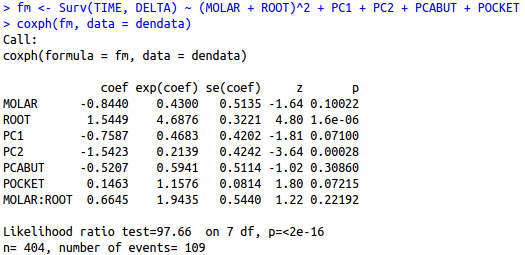
\includegraphics[width=4.68750in]{dental.png}
\caption{\texttt{coxph} output}
\end{figure}

\begin{enumerate}
\def\labelenumi{\alph{enumi}.}
\tightlist
\item
  (2 points) Suppose the log-partial likelihood for the model is
  -581.4417, what is the log-partial likelihood for the reduced model
  with no covariates?
\item
  (2 points) What is the hazard ratio that compares teeth with bridge
  adutment with those without? \label{pocket}
\item
  (2 points) What is the 95\% confidence interval for the hazard ratio
  in \#\ref{pocket}?
\item
  (2 points) What is the hazard ratio that compares teeth with nonbridge
  abutment and one proximal contacts with those with nonbridge abutment
  and two proximal contacts?
\item
  (2 points) What is the hazard ratio that compares molar teeth with
  non-molar teeth \textbf{among those underwent root canal treatment}?
\end{enumerate}

\textbf{\emph{Answer}}

\begin{enumerate}
\def\labelenumi{\alph{enumi}.}
\item
\end{enumerate}

\[G = 2 \cdot \{ l_p(\hat{\beta}) -l_p(0) \} \\ 
97.66 = 2 \cdot \{ -581.4417 -l_p(0) \} \\
l_p(0) = -630.2717\]

\begin{enumerate}
\def\labelenumi{\alph{enumi}.}
\setcounter{enumi}{1}
\item
  The hazard ratio that compares teeth with bridge adutment with those
  without is 0.5941.
\item
  \[exp[\hat{\beta} \pm 1.96 \cdot \widehat{SE}(\hat{\beta}) ] =  exp[-0.5207 \pm 1.96 \cdot 0.5114] = [0.218, 1.619]\]
\end{enumerate}

95\% confidence interval for the hazard ratio in \#\ref{b} is
\([0.218, 1.619]\).

\begin{enumerate}
\def\labelenumi{\alph{enumi}.}
\setcounter{enumi}{3}
\item
\end{enumerate}


\end{document}
